\clearpage

\section{Different performance metrics}\label{apx:metrics-review}

\todo{Keep? Review and copy-edit necessary.}

There are many different ways of evaluating the pipeline performance found in the field of pose estimation. Some of the evaluations include the following:
\begin{itemize}
\item Intersection over Union (IoU) of the object 3D cloud with a custom threshold classifying it as a good estimate or not (e.g. in the paper~\cite{10.1007/s11263-014-0733-5} the threshold score above 0.5 is considered good estimation).
\item Translation and rotation error between estimated 3D model and true 3D model with fixed thresholds (e.g. in the paper~\cite{shotton2013scene} they require the translation error to be below 5 cm and rotation error to be below 5\degree)
\item The average distance of all the points of the model from their transformed version, and if the error is less than the constant multiple of diameter of the 3D model, it is considered correctly evaluated (e.g. evaluation error is used in papers \cite{10.1007/978-3-642-37331-2_42, xiang2018posecnn})
\item Reprojection error that projects the estimated points onto the image and computes the pairwise distances in the image space, instead of computing distances in the 3D model space (e.g. used in paper~\cite{xiang2018posecnn})
\item The recovery error measured as Frobenius norm from estimated 3D model and true model, where 3D model is composed of 3D locations of important landmarks (e.g. elbow for human pose estimation)~\cite{wangni2018monocular}
\item Average Orientation Similarity (AOS) is the difference between the true and estimated model with a cosine similarity term~\cite{RedondoCabrera2016PoseEE}
\item Mean Angle Error (MAE) and Median Angle Error (MedError) evaluated and compared with other pose estimation error metrics in the paper~\cite{RedondoCabrera2016PoseEE}.
\end{itemize}

\section{Sampling of orientations}\label{apx:orientation-sampling}

\figref{uniform-orientations} shows some properties of a uniform distribution of orientations over $\SO(3)$.
\figref{uniform-angles} shows a non-uniform distribution of orientations---created by sampling Euler angles uniformly---that might happen in real cryo-EM acquisitions.
\mdeff{Should we use a single color for all plots if they don't require different colors to be understood?}

\begin{figure}[ht!]
    \centering
    \begin{subfigure}[b]{0.30\linewidth}
        \centering
        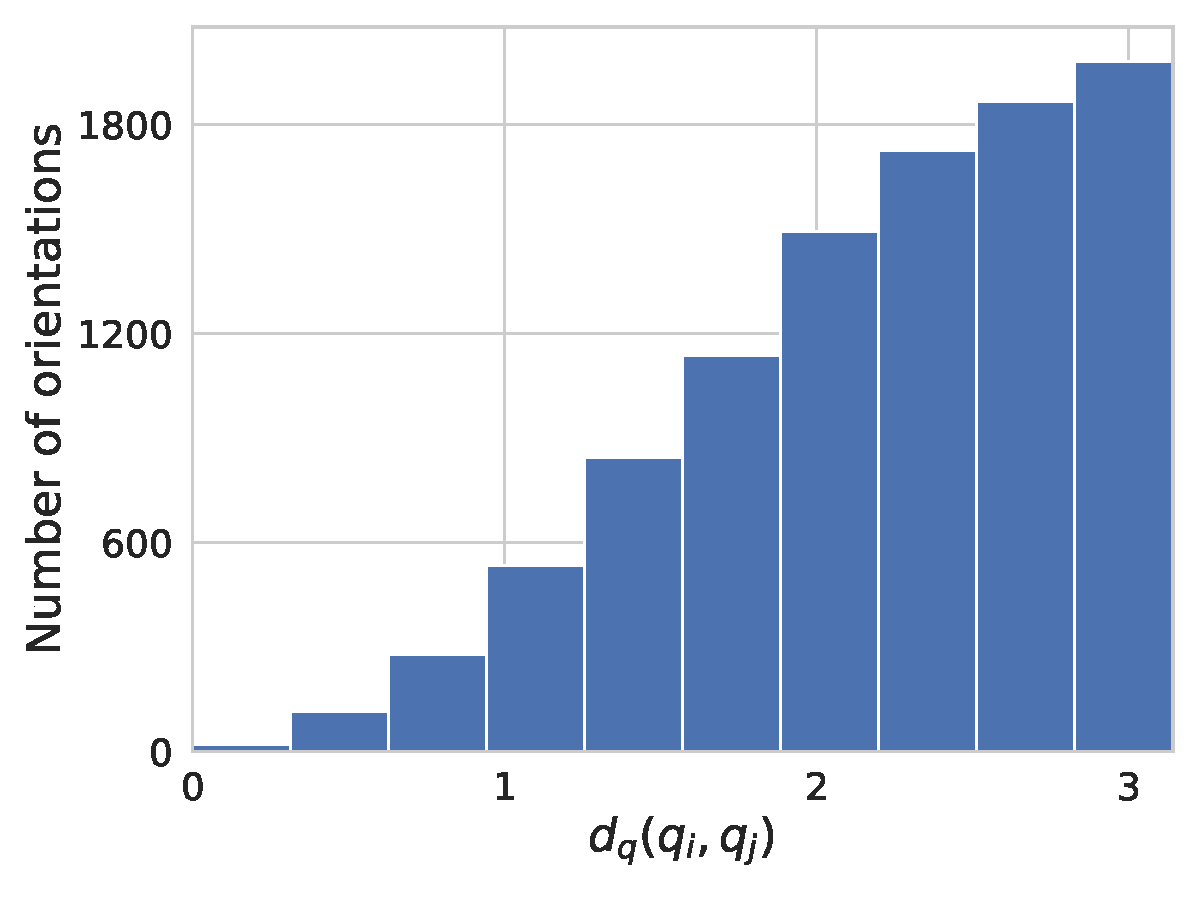
\includegraphics[height=8em]{figures/dQ_5j0n_uniform_quaternions.pdf}
        \caption{Distribution of ($10,000<P^2$) distances.}
    \end{subfigure}
    \hfill
    \begin{subfigure}[b]{0.66\linewidth}
        \centering
        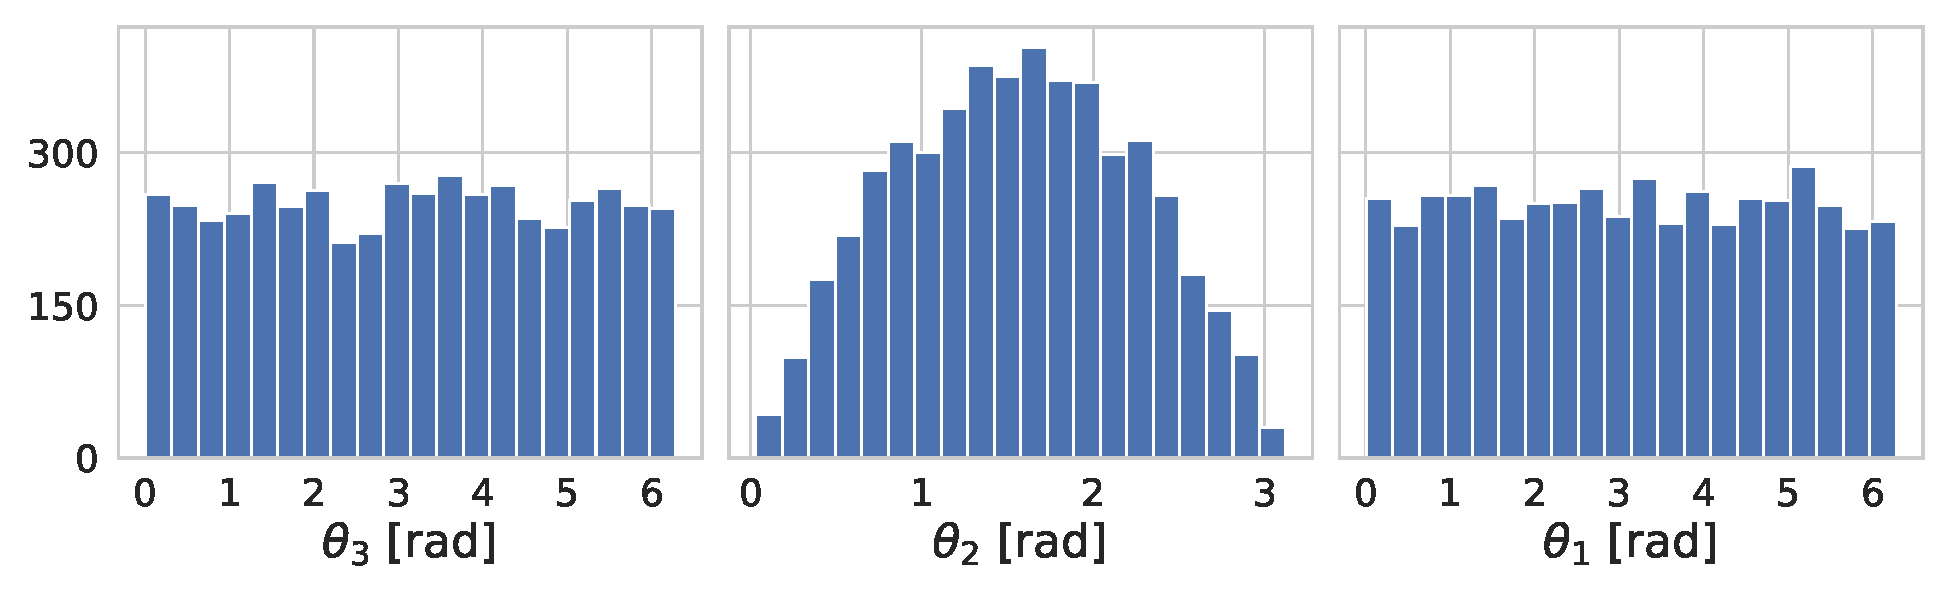
\includegraphics[height=8em]{figures/uniform_quaternions_ang.pdf}
        \caption{Distribution of Euler angles $\bth = (\theta_3,\theta_2,\theta_1)$.}
    \end{subfigure}
    \\ \vspace{1em}
    \begin{subfigure}[b]{0.30\linewidth}
        \centering
        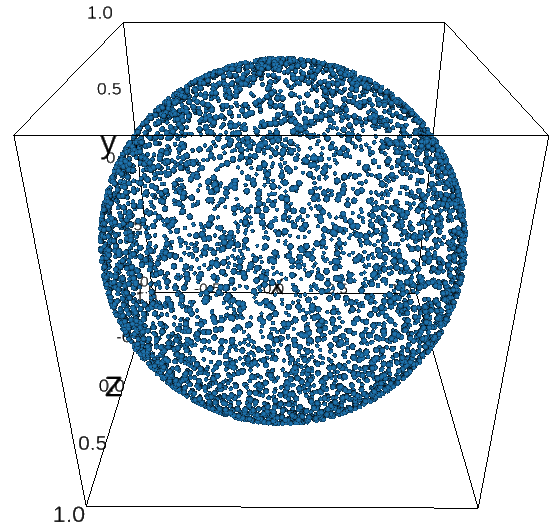
\includegraphics[height=8em]{figures/uniform_quaternion.png}
        \caption{Sampled directions $(\theta_2, \theta_1)$.}
    \end{subfigure}
    \hfill
    \begin{subfigure}[b]{0.66\linewidth}
        \centering
        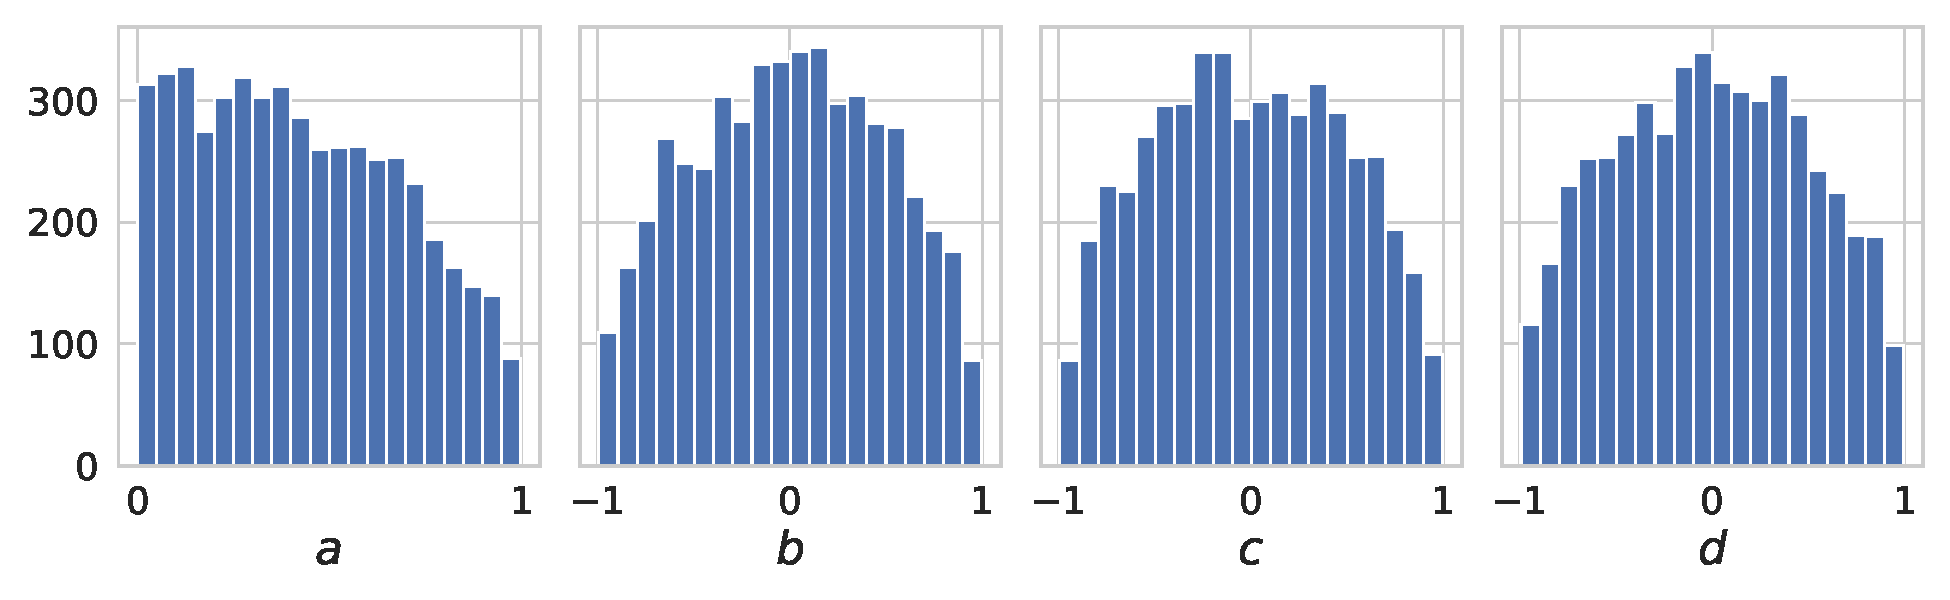
\includegraphics[height=8em]{figures/uniform_quaternions_q.pdf}
        \caption{Distribution of quaternions $q = a + b\boldsymbol{i} + c\boldsymbol{j} + d\boldsymbol{k}$.}
    \end{subfigure}
    \caption{%
        Uniform sampling of $P=5,000$ orientations from $\SO(3)$.
        \mdeff{That's not uniform in quaternion space, as shown by (d). ;) It's uniform in rotation / SO(3) space. How did you sample it? A classic way is to draw from $\mathcal{N}(0, I_4)$ then normalize to unit norm. More at \url{https://mathworld.wolfram.com/SpherePointPicking.html}.}
        }\label{fig:uniform-orientations}
\end{figure}

\begin{figure}[ht!]
    \centering
    \begin{subfigure}[b]{0.36\linewidth}
        \centering
        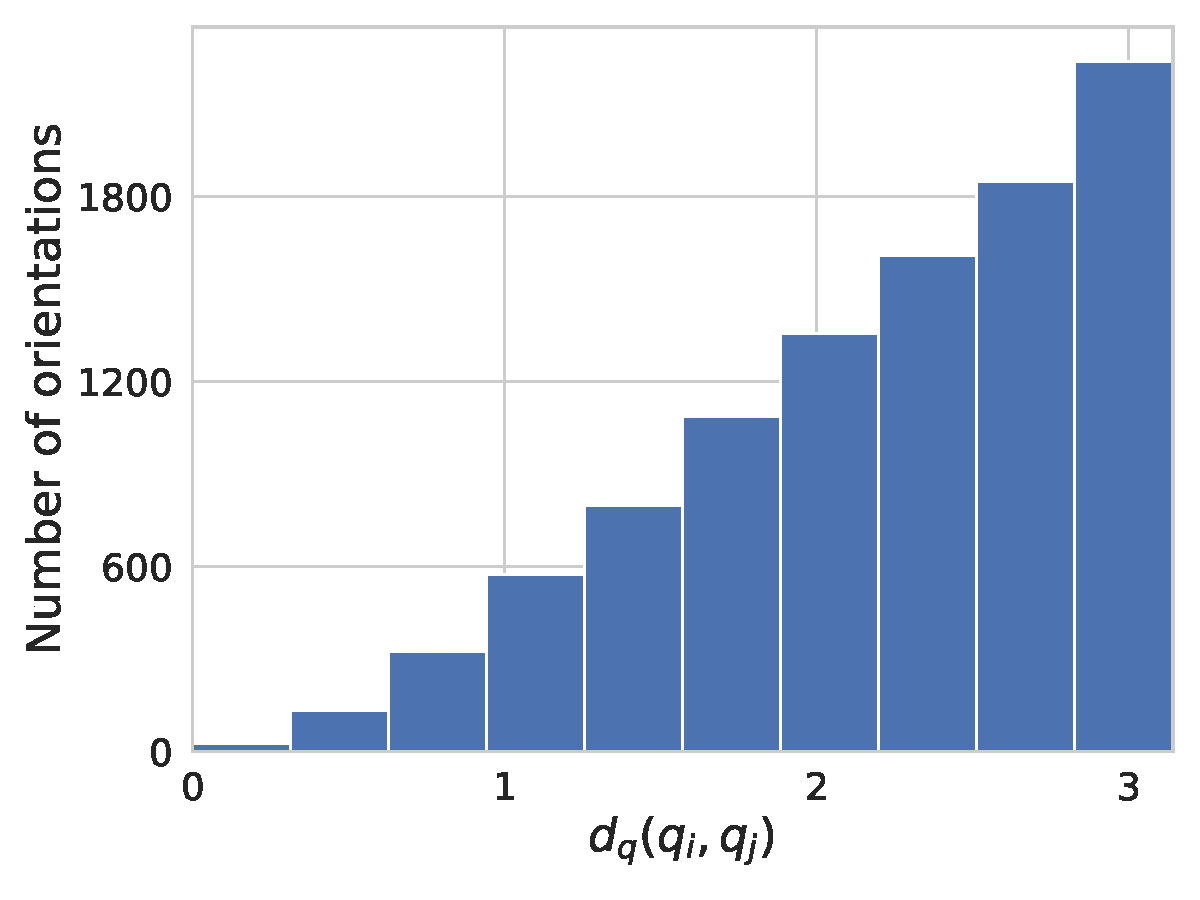
\includegraphics[height=8em]{figures/dQ_5j0n_uniform_angles.pdf}
        \caption{Distribution of ($10,000<P^2$) distances.}
    \end{subfigure}
    \hfill
    \begin{subfigure}[b]{0.62\linewidth}
        \centering
        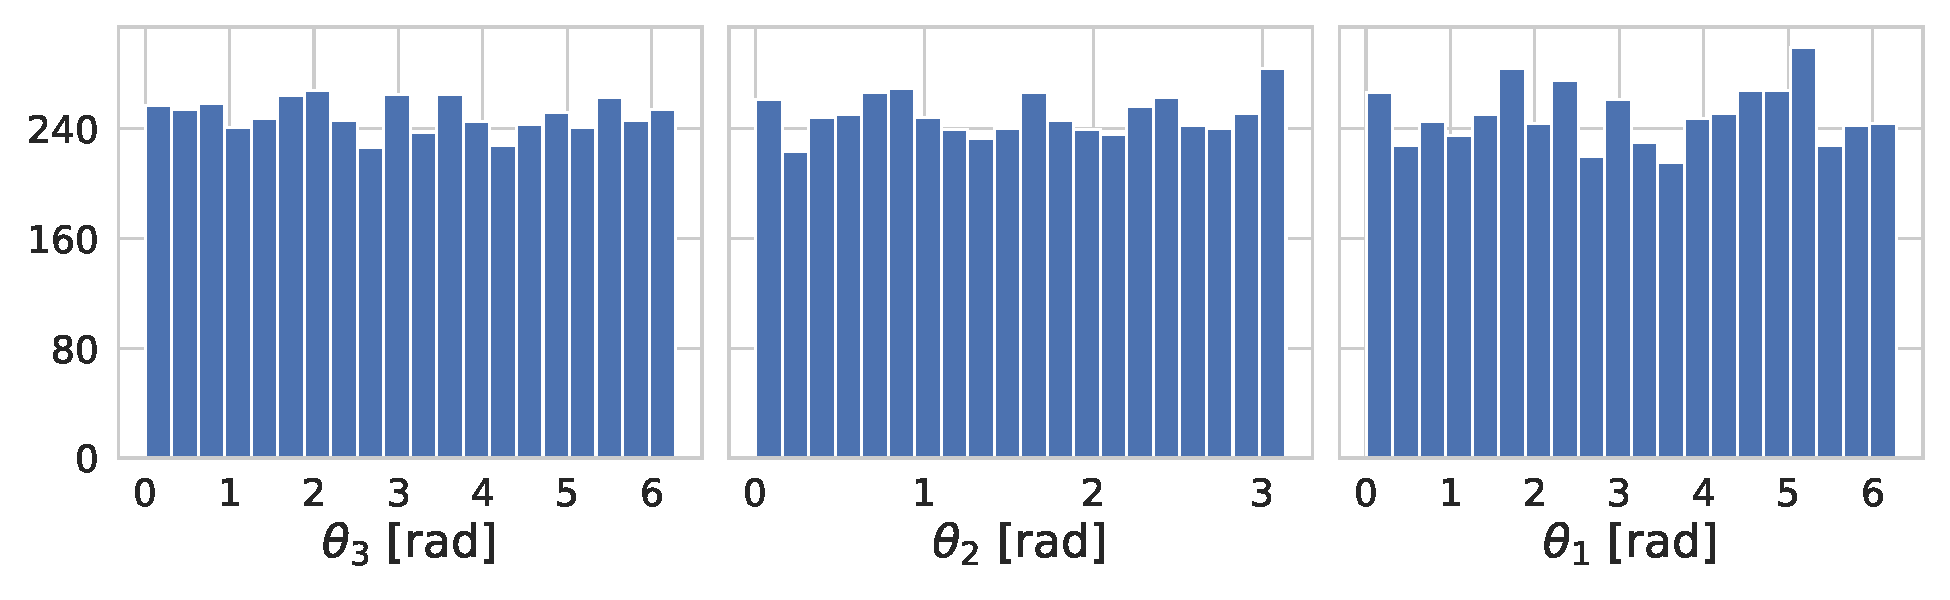
\includegraphics[height=8em]{figures/uniform_angles_ang.pdf}
        \caption{Distribution of Euler angles $\bth = (\theta_3,\theta_2,\theta_1)$.}
    \end{subfigure}
    \\ \vspace{1em}
    \begin{subfigure}[b]{0.30\linewidth}
        \centering
        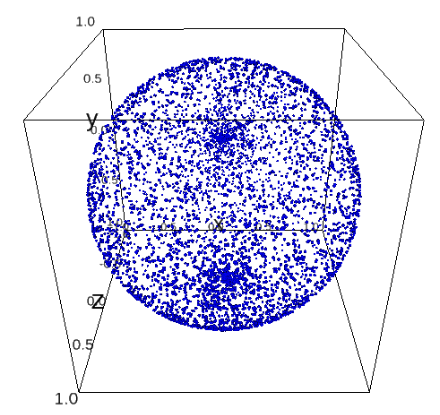
\includegraphics[height=8em]{figures/uniform_angles.png}
        \caption{Sampled directions $(\theta_2, \theta_1)$.}
    \end{subfigure}
    \hfill
    \begin{subfigure}[b]{0.66\linewidth}
        \centering
        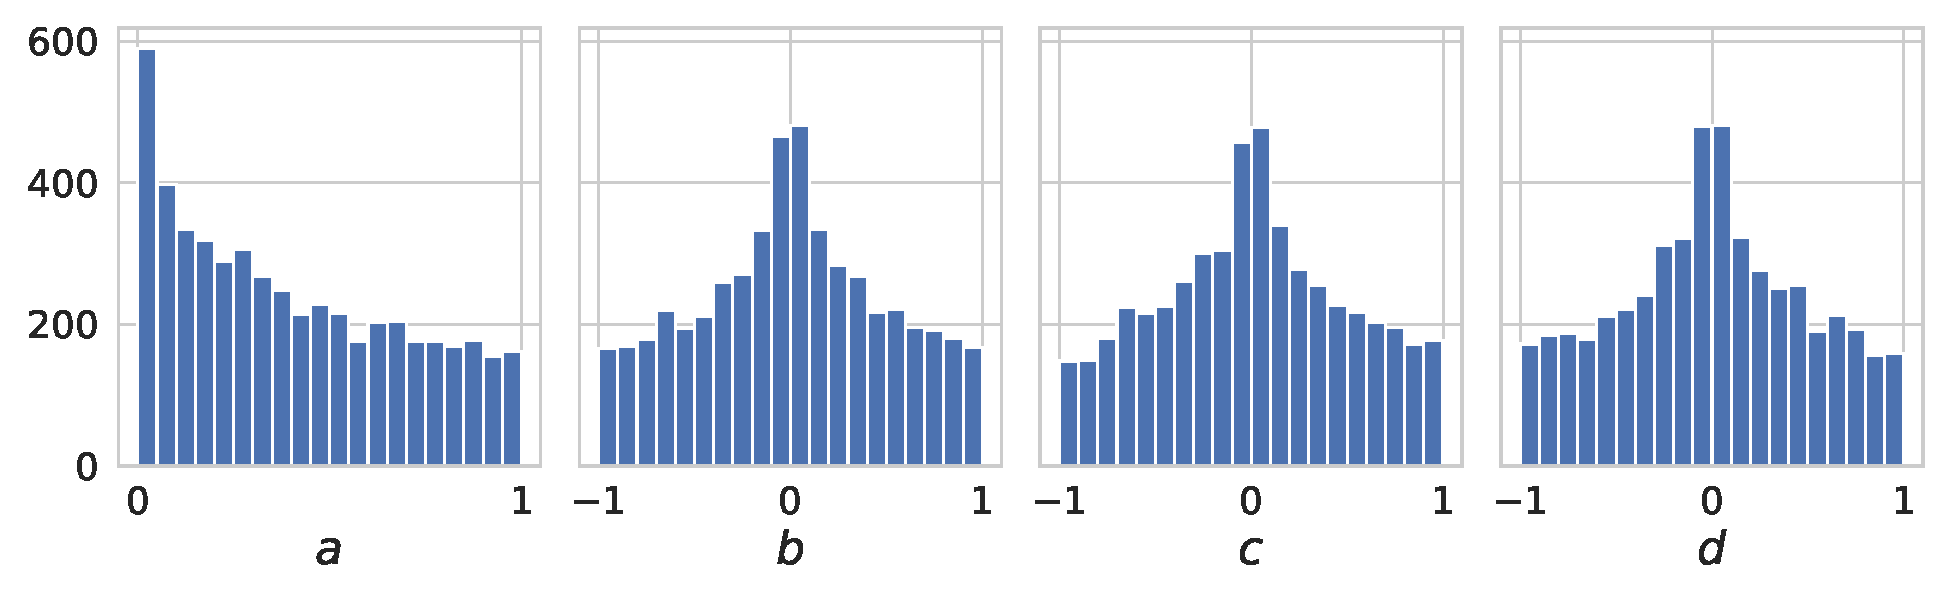
\includegraphics[height=8em]{figures/uniform_angles_q.pdf}
        \caption{Distribution of quaternions $q = a + b\boldsymbol{i} + c\boldsymbol{j} + d\boldsymbol{k}$.}
    \end{subfigure}
     \caption{%
        Uniform sampling of $P=5,000$ Euler angles from $[0,2\pi[ \, \times \, [0,\pi] \times [0,2\pi[$ inducing a non-uniform distribution of orientations.
        }\label{fig:uniform-angles}
\end{figure}

\figref{orientation-constraints} shows distributions of induced distances when directions $(\theta_2, \theta_1)$ are constrained to an half (to learn from asymmetric proteins like \texttt{5j0n}) or a quarter (e.g., for proteins with D2 symmetry like \texttt{5a1a}) of the 2-sphere.
Observe that while the distributions flatten (compare with Figures~\ref{fig:uniform-orientations},\ref{fig:uniform-angles}a), the shorter distances are still way under-sampled.

\begin{figure}[ht!]
    \centering
    \begin{subfigure}[b]{0.22\linewidth}
        \centering
        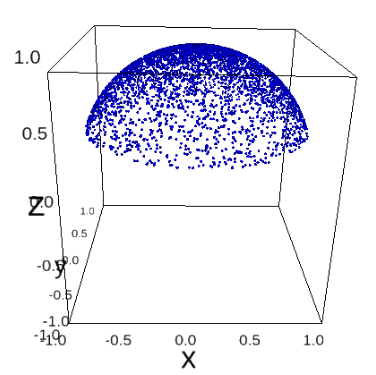
\includegraphics[height=7em]{figures/5j0n-half.png}
        \caption{Directions sampled from \todo{$(\theta_2, \theta_1) \in [0,\frac{\pi}{2}[ \, \times \, [0,2\pi[$}, an half of the 2-sphere.}
    \end{subfigure}
    \hfill
    \begin{subfigure}[b]{0.22\linewidth}
        \centering
        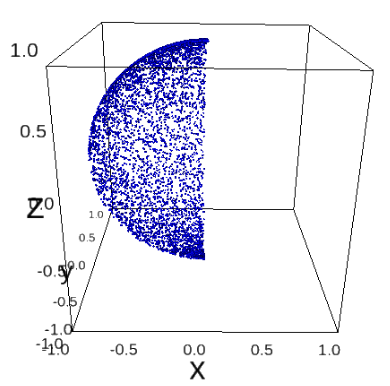
\includegraphics[height=7em]{figures/5a1a_quarter.png}
        \caption{Directions sampled from $(\theta_2, \theta_1) \in [0,\pi[ \, \times \, [0,\frac{\pi}{2}[$, a quarter of the 2-sphere.}
    \end{subfigure}
    \hfill
    \begin{subfigure}[b]{0.22\linewidth}
        \centering
        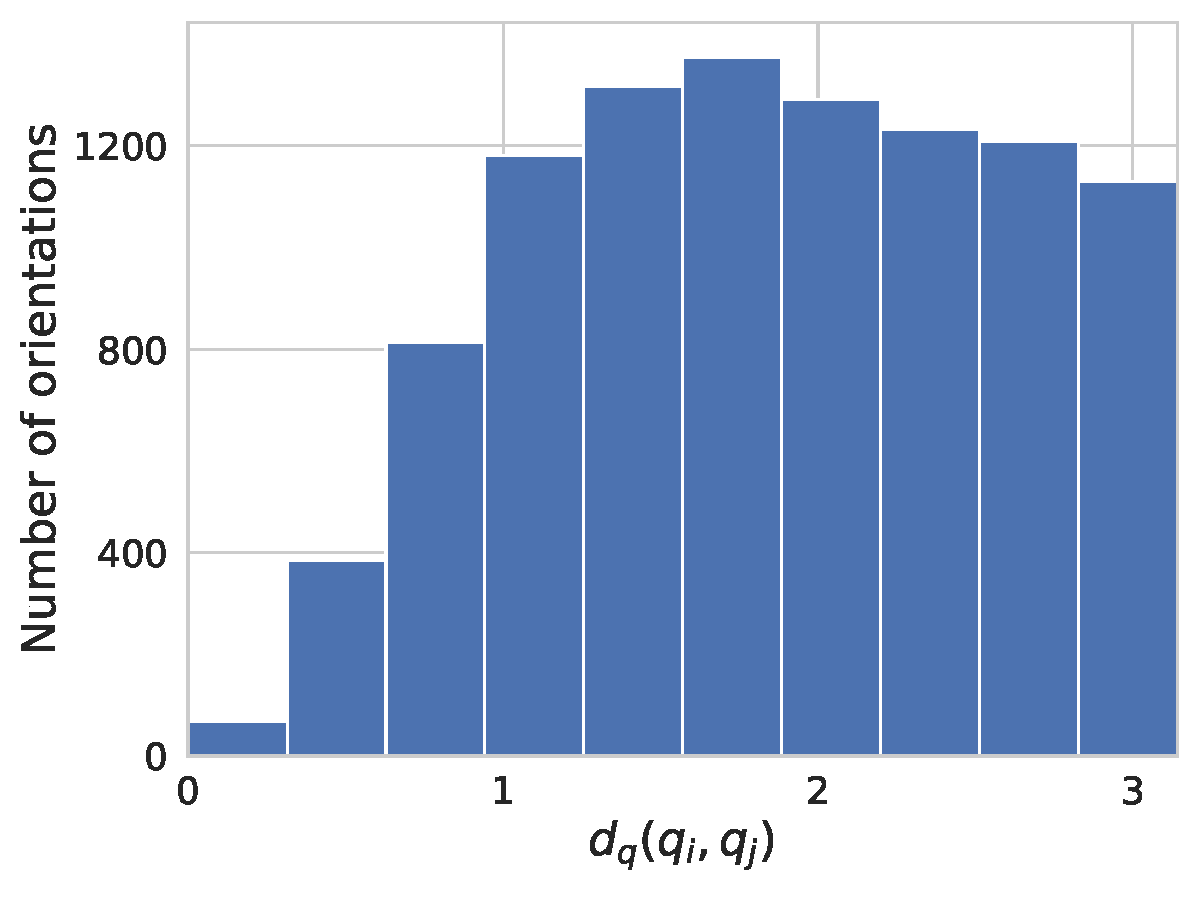
\includegraphics[height=7em]{figures/dQ_5j0n_half.pdf}
        \caption{Induced distribution of distances (half).}
    \end{subfigure}
    \hfill
    \begin{subfigure}[b]{0.22\linewidth}
        \centering
        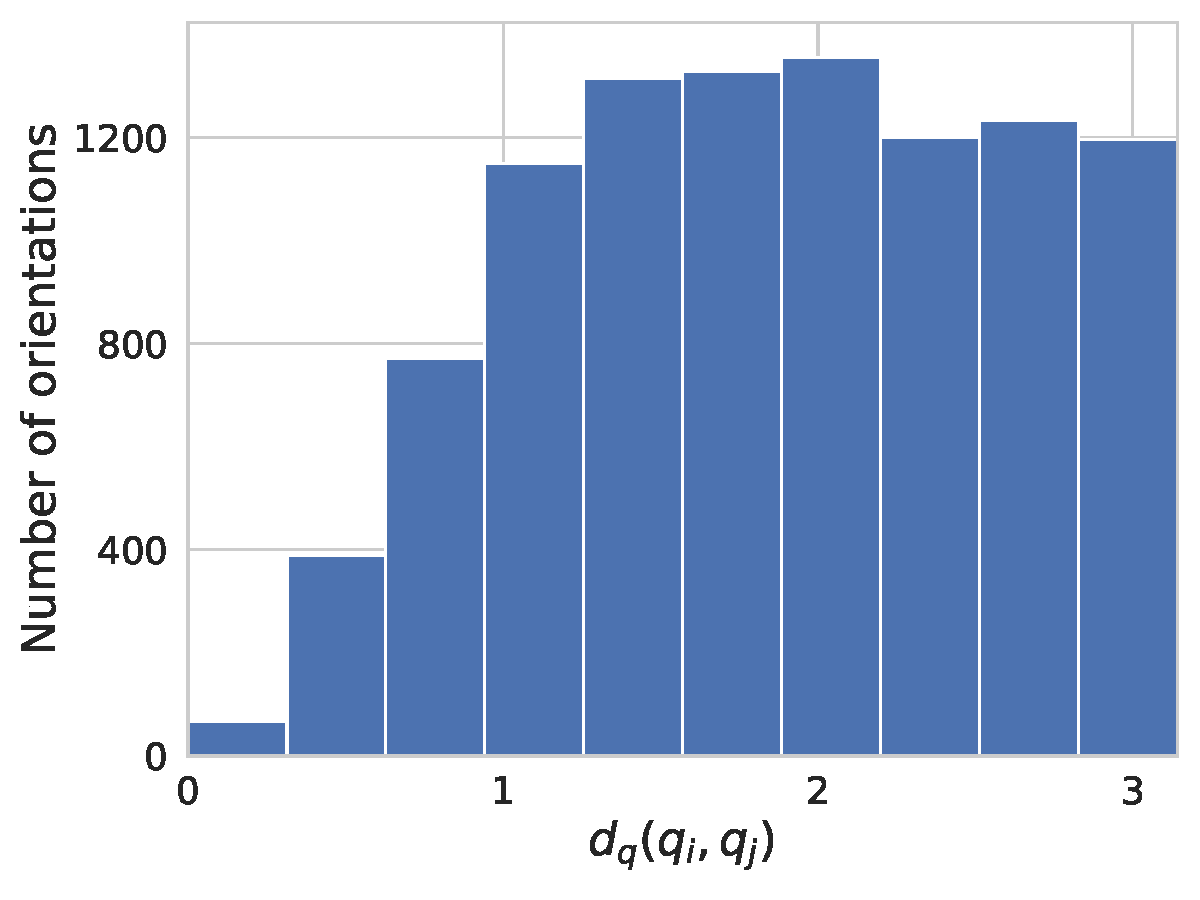
\includegraphics[height=7em]{figures/dQ_5a1a_quarter.pdf}
        \caption{Induced distribution of distances (quarter).}
    \end{subfigure}
    \caption{%
        Distributions of $P=5,000$ directions $(\theta_2, \theta_1)$ as points on the 2-sphere (see also \figref{imaging-geometry}), illustrating their constrained range, and the distances they induce.
        \todo{Make the difference between half and quarter coverage clearer.}
        \mdeff{Have a single histogram with two colors? They are mostly the same, and we could save space.}
        }\label{fig:orientation-constraints}
\end{figure}

\section{Orientation recovery from exact distances}\label{apx:results:orientation-recovery:exact}

%\mdeff{Story: works perfectly despite no convexity guarantee and sampling.}

\lau{Smooth.}
To verify that the lack of a convexity guarantee for \eqnref{orientation-recovery} and the sampling of the sum are non-issues in practice, we attempted orientation recovery under exact distance estimation $d_p(\p_i, \p_j) = d_q(q_i, q_j)$.
Orientations were perfectly recovered.
\figref{5j0n-orientation-recovery-loss} shows the convergence of the loss $L_\text{OR}$ to zero.
\figref{5j0n-aa-loss-perfect-distances} shows how~\eqnref{orientation-recovery-error} could then perfectly align the recovered and true orientations---leading to $E_\text{OR} = 0$.
% Demonstrating that alignment is necessary to evaluate the performance of orientation recovery.

\begin{figure}[ht!]
    \begin{minipage}[t]{0.27\linewidth}
        \centering
        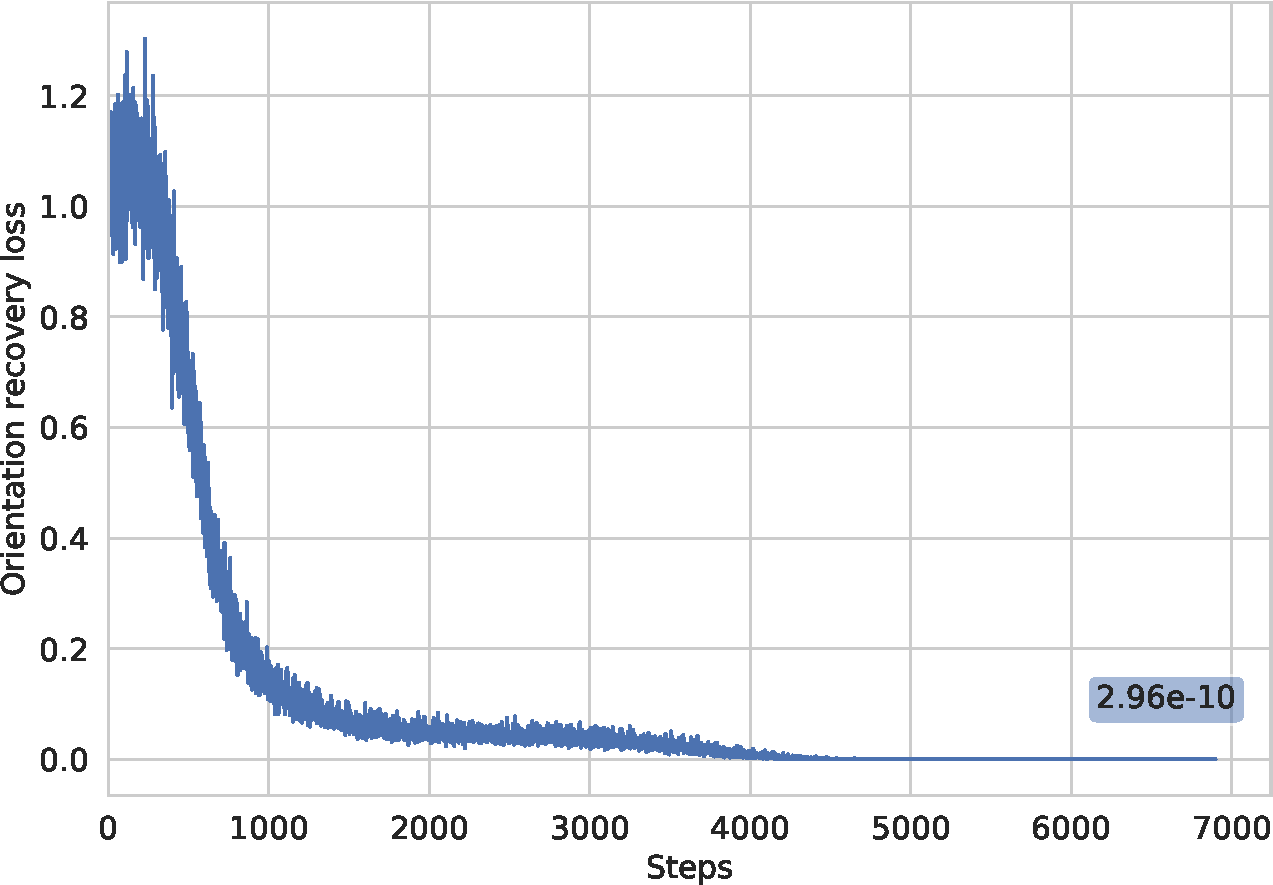
\includegraphics[height=3cm]{figures/5j0n_perfect_angle_recovery}
        \caption{%
            Example of perfect orientation recovery (for \texttt{5j0n}).
            The loss $L_\text{OR}$ \eqnref{orientation-recovery} converges to zero when the distance estimation is perfect, i.e., $d_p(\p_i, \p_j) = d_q(q_i, q_j)$.
            \todo{Add $L_\text{OR}$ to the y-axis label and blue box.}
        }\label{fig:5j0n-orientation-recovery-loss}
    \end{minipage}
    \hfill
    \begin{minipage}[t]{0.70\linewidth}
%        \begin{subfigure}[b]{0.19\linewidth}
%            \centering
%            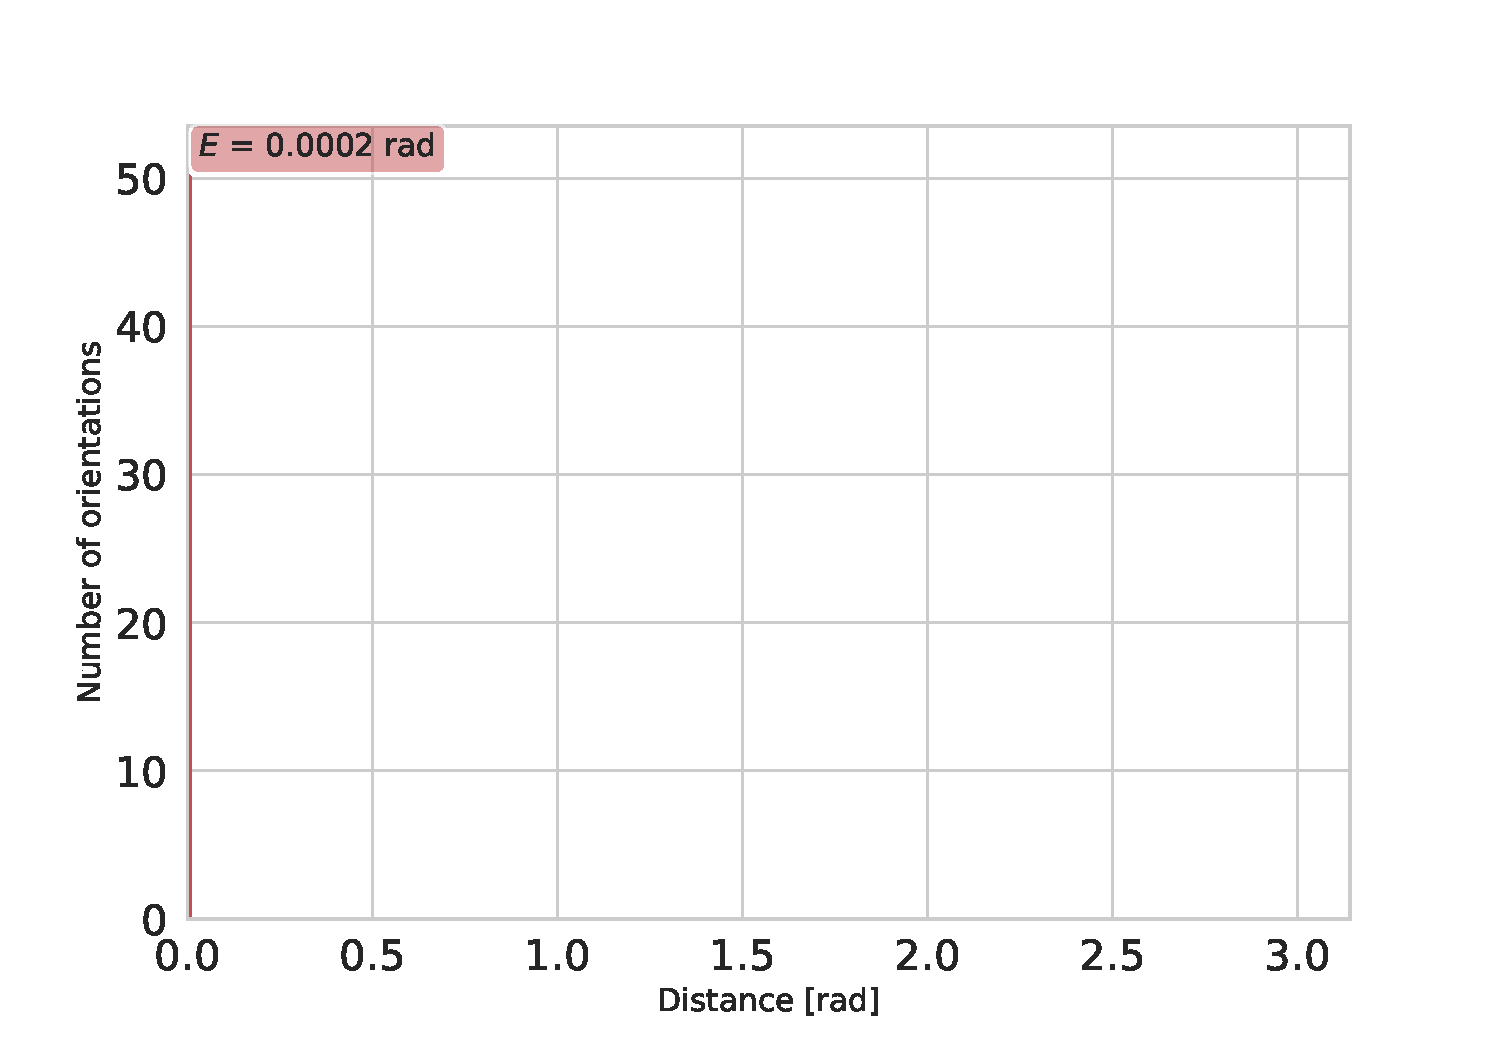
\includegraphics[height=3cm]{figures/5j0n_perfect_angle_ralignment_after}
%            \caption{Orientation recovery error with alignment.}
%        \end{subfigure}
%        \hfill
        \begin{subfigure}[t]{4.3cm}
            \centering
            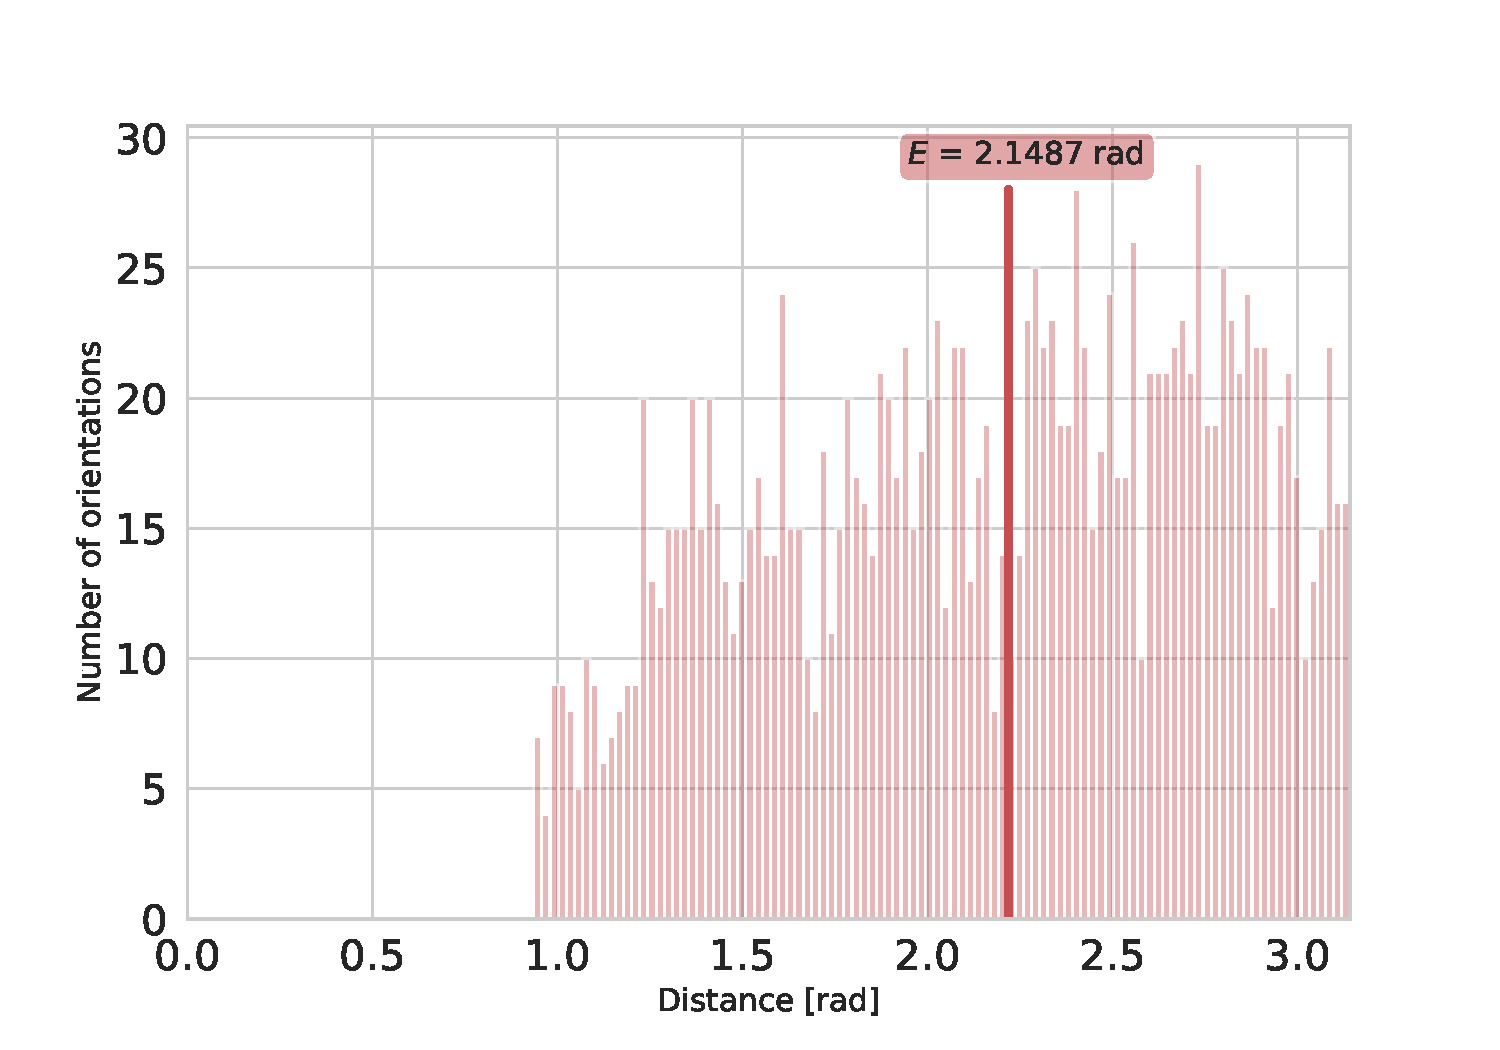
\includegraphics[height=3cm]{figures/5j0n_perfect_angle_ralignment_before}
            \caption{Error histogram $\{ d_q (q_i, \widehat{q_i}) \}$, i.e., before alignment.}
        \end{subfigure}
        \hfill
        \begin{subfigure}[t]{3.4cm}
            \centering
            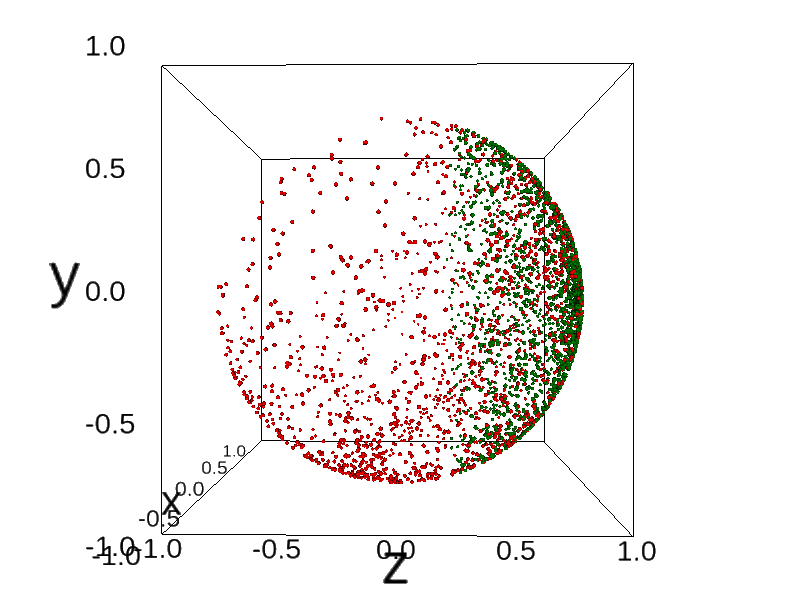
\includegraphics[height=3cm]{figures/coverage_alignment_before.png}
            \caption{Orientations before alignment.}
        \end{subfigure}
        \hfill
        \begin{subfigure}[t]{3.4cm}
            \centering
            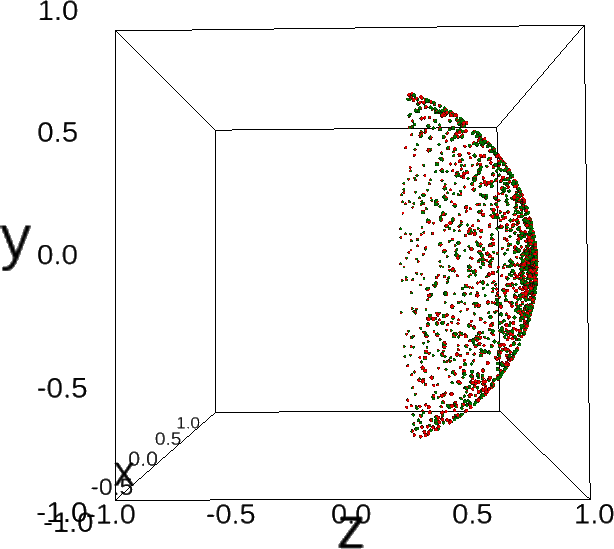
\includegraphics[height=3cm]{figures/coverage_alignment_after.png}
            \caption{Orientations after alignment.}
        \end{subfigure}
        \caption{%
            Example of perfect alignment~\eqnref{orientation-recovery-error} after a perfect orientation recovery~\eqnref{orientation-recovery}.
            (a)~shows the error before alignment.
            % and $\T$ as the optimum of \eqnref{orientation-recovery-error} on the right.
            (b-c)~show the orientations projected on $\mathbb{S}^2 \subset \SO(3)$ before (b) and after (c) alignment.
            Green points are the true orientations $\{q_i\}$ and red points are the recovered orientations $\{\widehat{q_i}\}$.
            % The Figure (b) is exactly aligned which can be seen when zoomed. Due to plotting artifacts,
            While both colors are seen in (c), they are exactly superimposed.
        }\label{fig:5j0n-aa-loss-perfect-distances}
    %    \label{fig:angle-alignment-perfect}
    \end{minipage}
\end{figure}

\section{Euclidean distance between projections}\label{apx:results:distance-estimation}
% Orientation distance as, Estimating distances with

%\mdeff{Story: simplest baseline estimator, $d_{pe}$ somewhat estimates $d_q$, quickly plateaus (even in the simplest noiseless and centered case).
%Note the difference between symmetric and asymmetric proteins.}

\begin{itemize}
    \item \mdeff{Jelena: from which coverage were the projections sampled from here?}
    \item \todo{Copy-edit.}
\end{itemize}

We evaluate $d_p(\p_i, \p_j) = \Vert \p_i - \p_j \Vert_2$ (i.e., the Euclidean distance) as a baseline distance estimator.
From $P = 5,000$ possible projection, we randomly select $5$ projections.
For each of these projections, we compute the Euclidean distance between aforementioned projection and all the others $d_p(\mathbf{p}_i,\mathbf{p}_j)=\lVert\mathbf{p}_i-\mathbf{p}_j\rVert_2$ and their corresponding orientation distance $d_q(q_i,q_j)$ through~\eqnref{distance:orientations}.
We then report the $(d_q,d_p)$ relationship for all pairs in \figref{euclidean-not-robust}, for both the \texttt{5j0n} (left) and \texttt{5a1a} (right).

Two principal observations can be made from this experiment.
First, as suspected, $d_p$ fails to be a consistent predictor of $d_q$, even in the simple imaging conditions considered here (no noise, no shift, no PSF).
In particular, the larger the quaternion distance $d_q$, the poorer the predictive ability of $d_p$ (the plot plateaus).
The other interesting observation is that the trend of $(d_q,d_p)$ plot of the \texttt{5a1a} appears to take symmetric shape of letter \texttt{M} which can be explained with the fact that this protein has intrinsic dihedral (D2) symmetry~\cite{noauthor_d2sym_nodate,noauthor_5a1asym_nodate}.
\mdeff{Check these refs. Other ones are used in main text?}

\begin{figure}[ht!]
    \begin{minipage}[t]{0.55\linewidth}
        \begin{subfigure}[t]{0.48\textwidth}
            \centering
            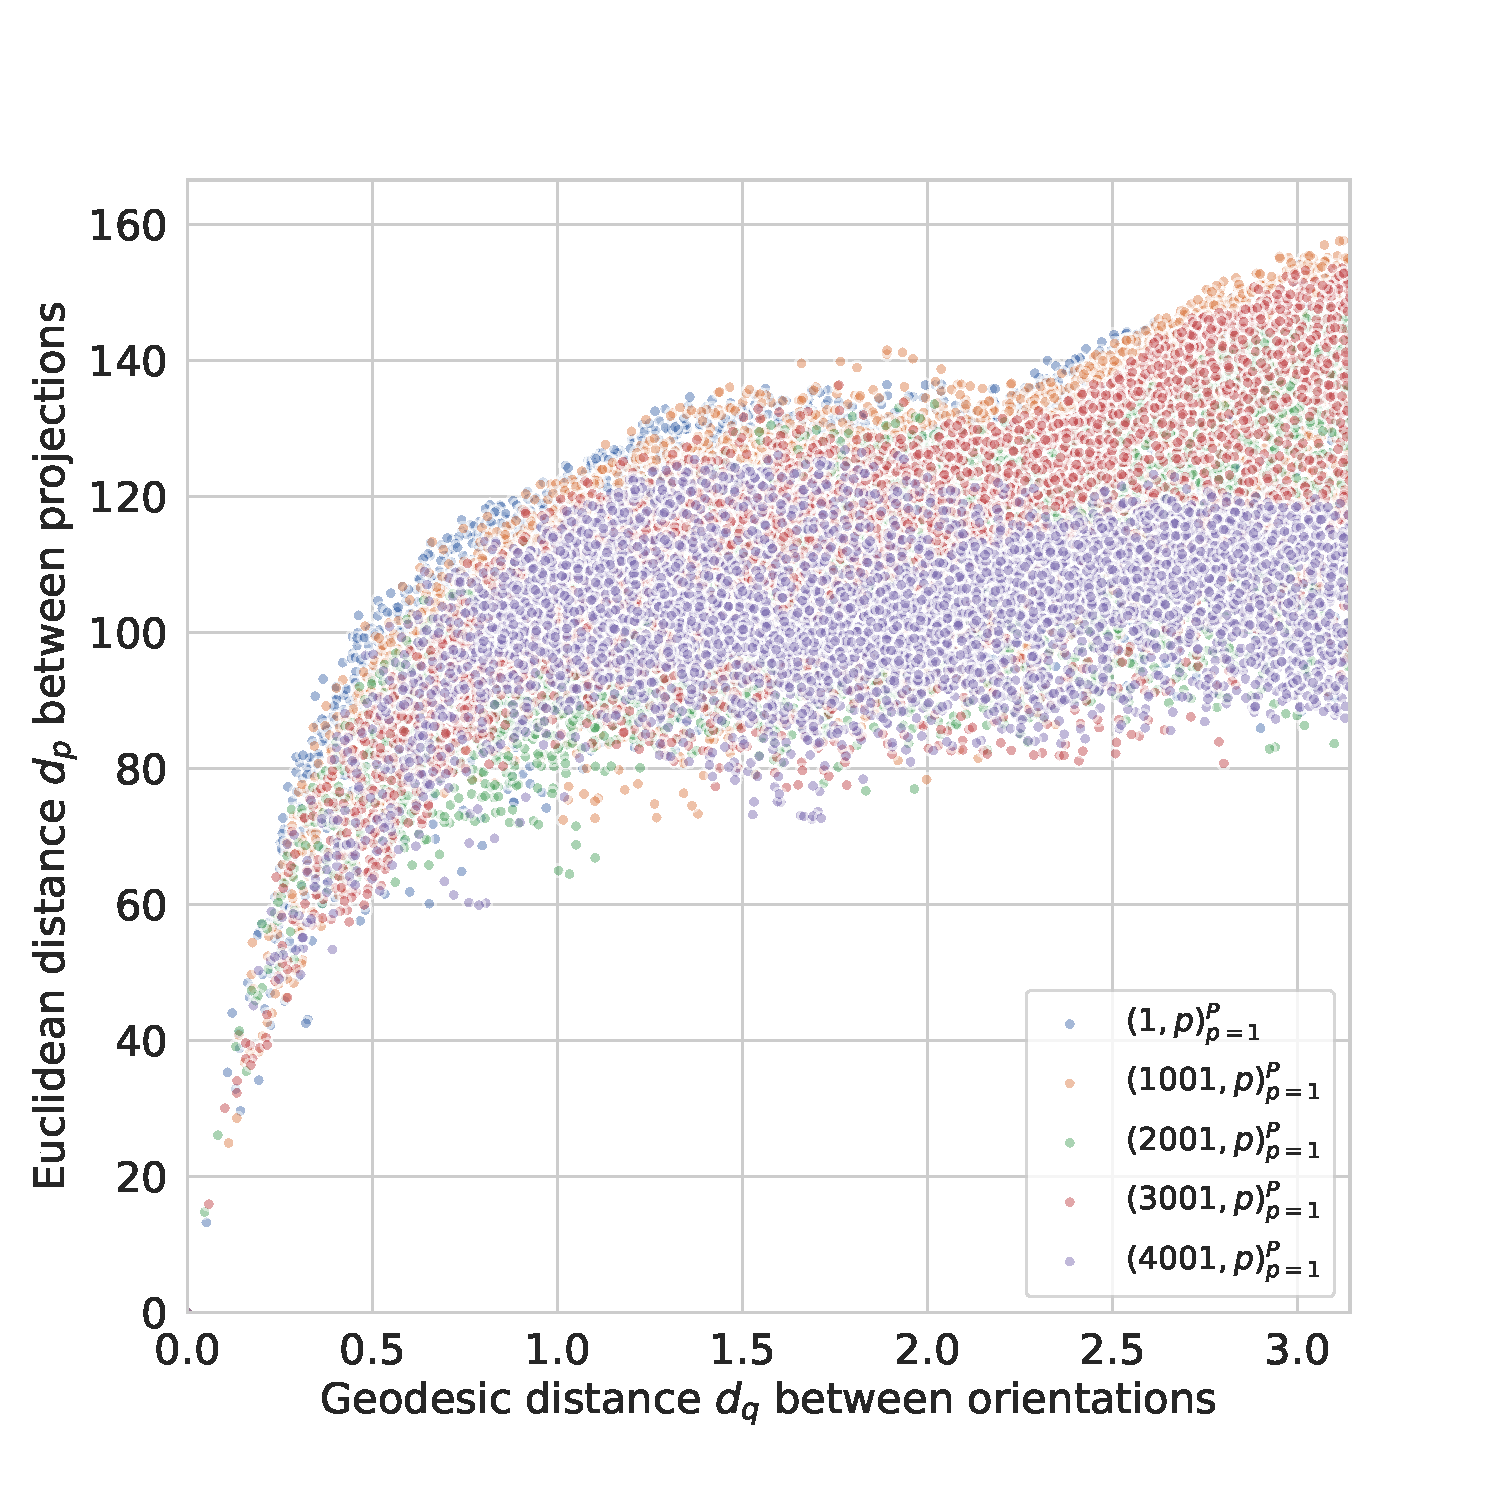
\includegraphics[height=4cm]{figures/eucl_notrobust_5j0n}
            \caption{\texttt{5j0n}}
        \end{subfigure}
        \hfill
        \begin{subfigure}[t]{0.48\textwidth}
            \centering
            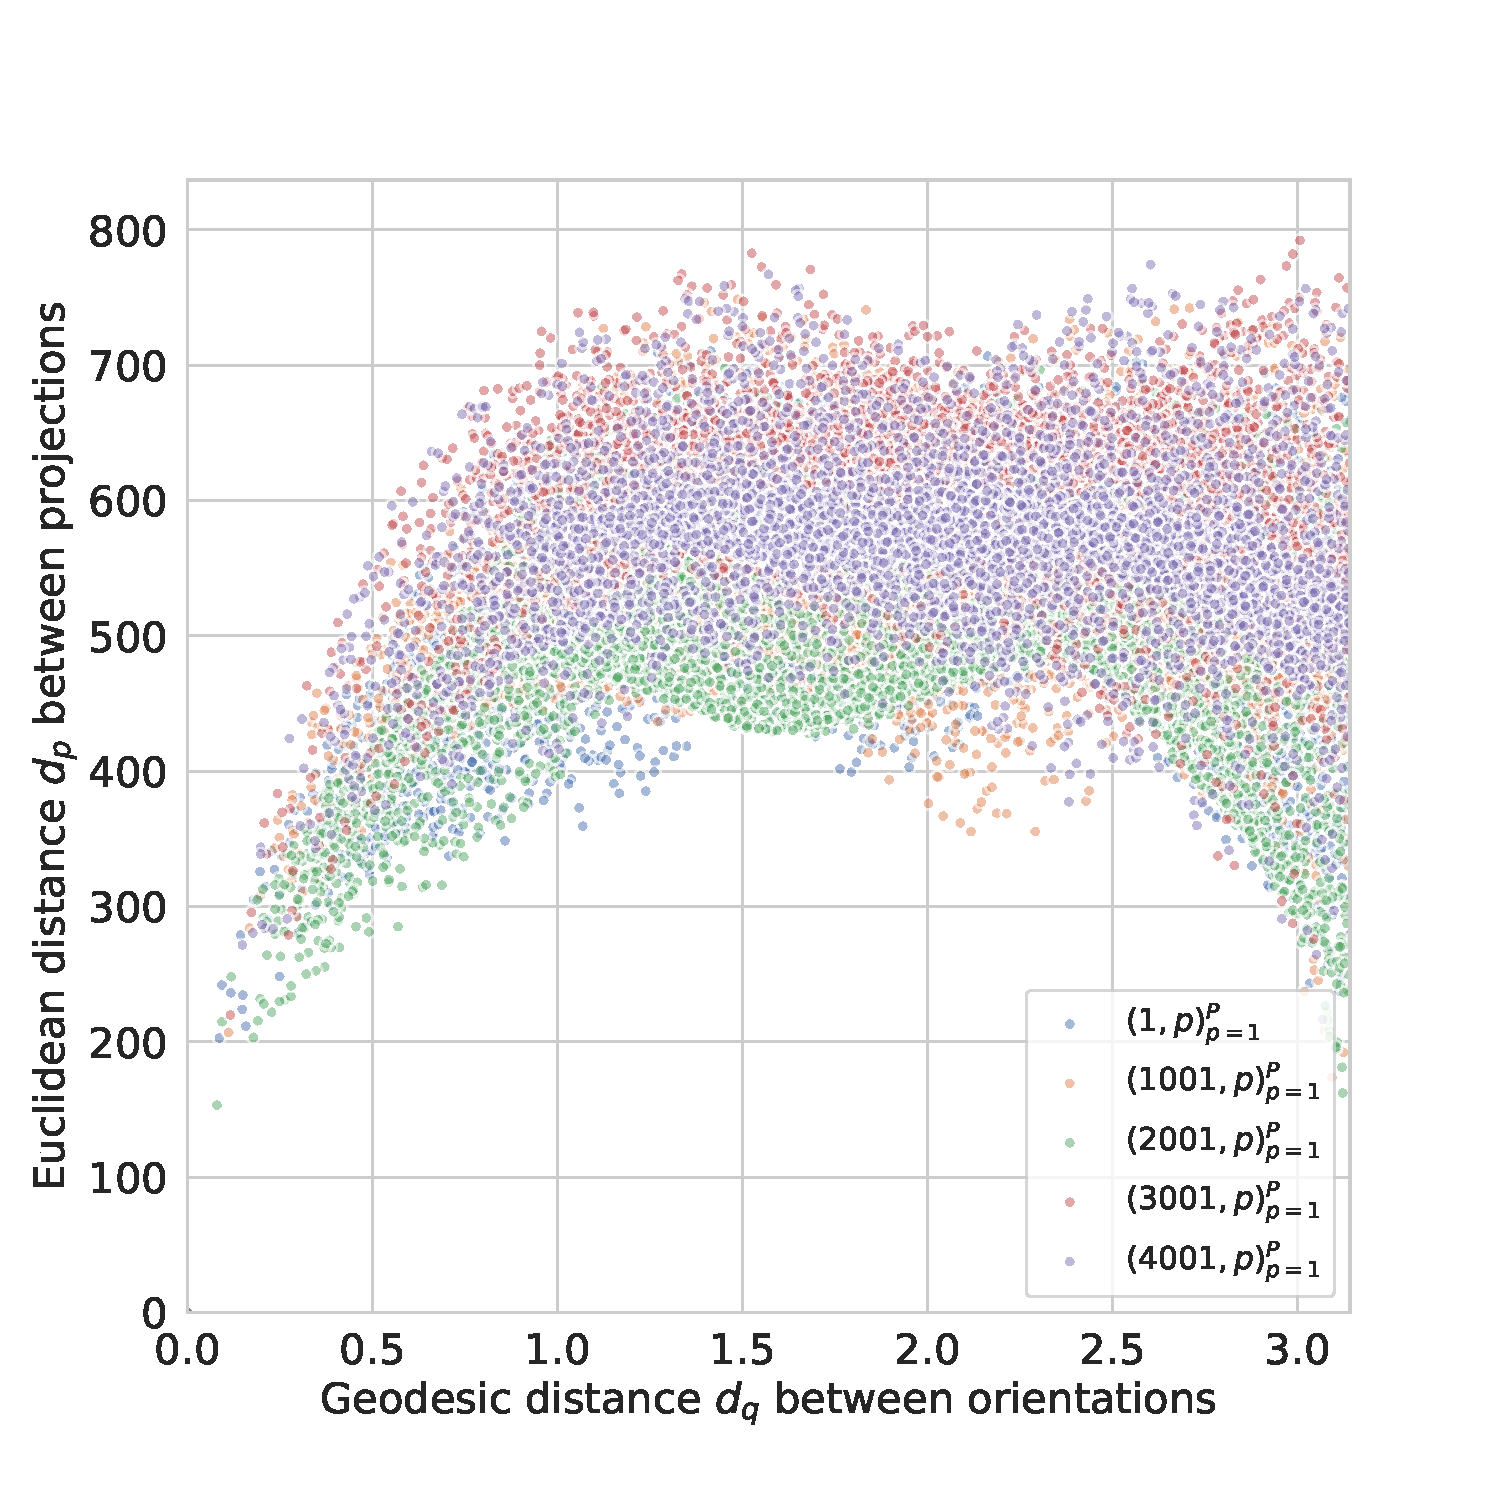
\includegraphics[height=4cm]{figures/eucl_notrobust_5a1a}
            \caption{\texttt{5a1a}}\label{fig:euclidean-not-robust:5a1a}
        \end{subfigure}
        \caption{%
            The Euclidean distance between two projections $d_p(\p_i, \p_j) = \Vert \p_i - \p_j \Vert_2$ versus their actual relative orientation $d_q(q_i, q_j)$ with the half-sphere direction coverage.
            Each color represent the distances between one fixed projection and the other $P-1$ projections.
    %        The color corresponds to projection pairs that share one projection, i.e., distance between one projection with all other projections.
            While there is some correlation, especially at small distances, the Euclidean distance is a poor estimator.
            Because \texttt{5a1a} has D2 symmetries, two projections might be identical while not having been acquired from the same orientation.
        }\label{fig:euclidean-not-robust}
    \end{minipage}
    \hfill
    \begin{minipage}[t]{0.4\linewidth}
        \centering
        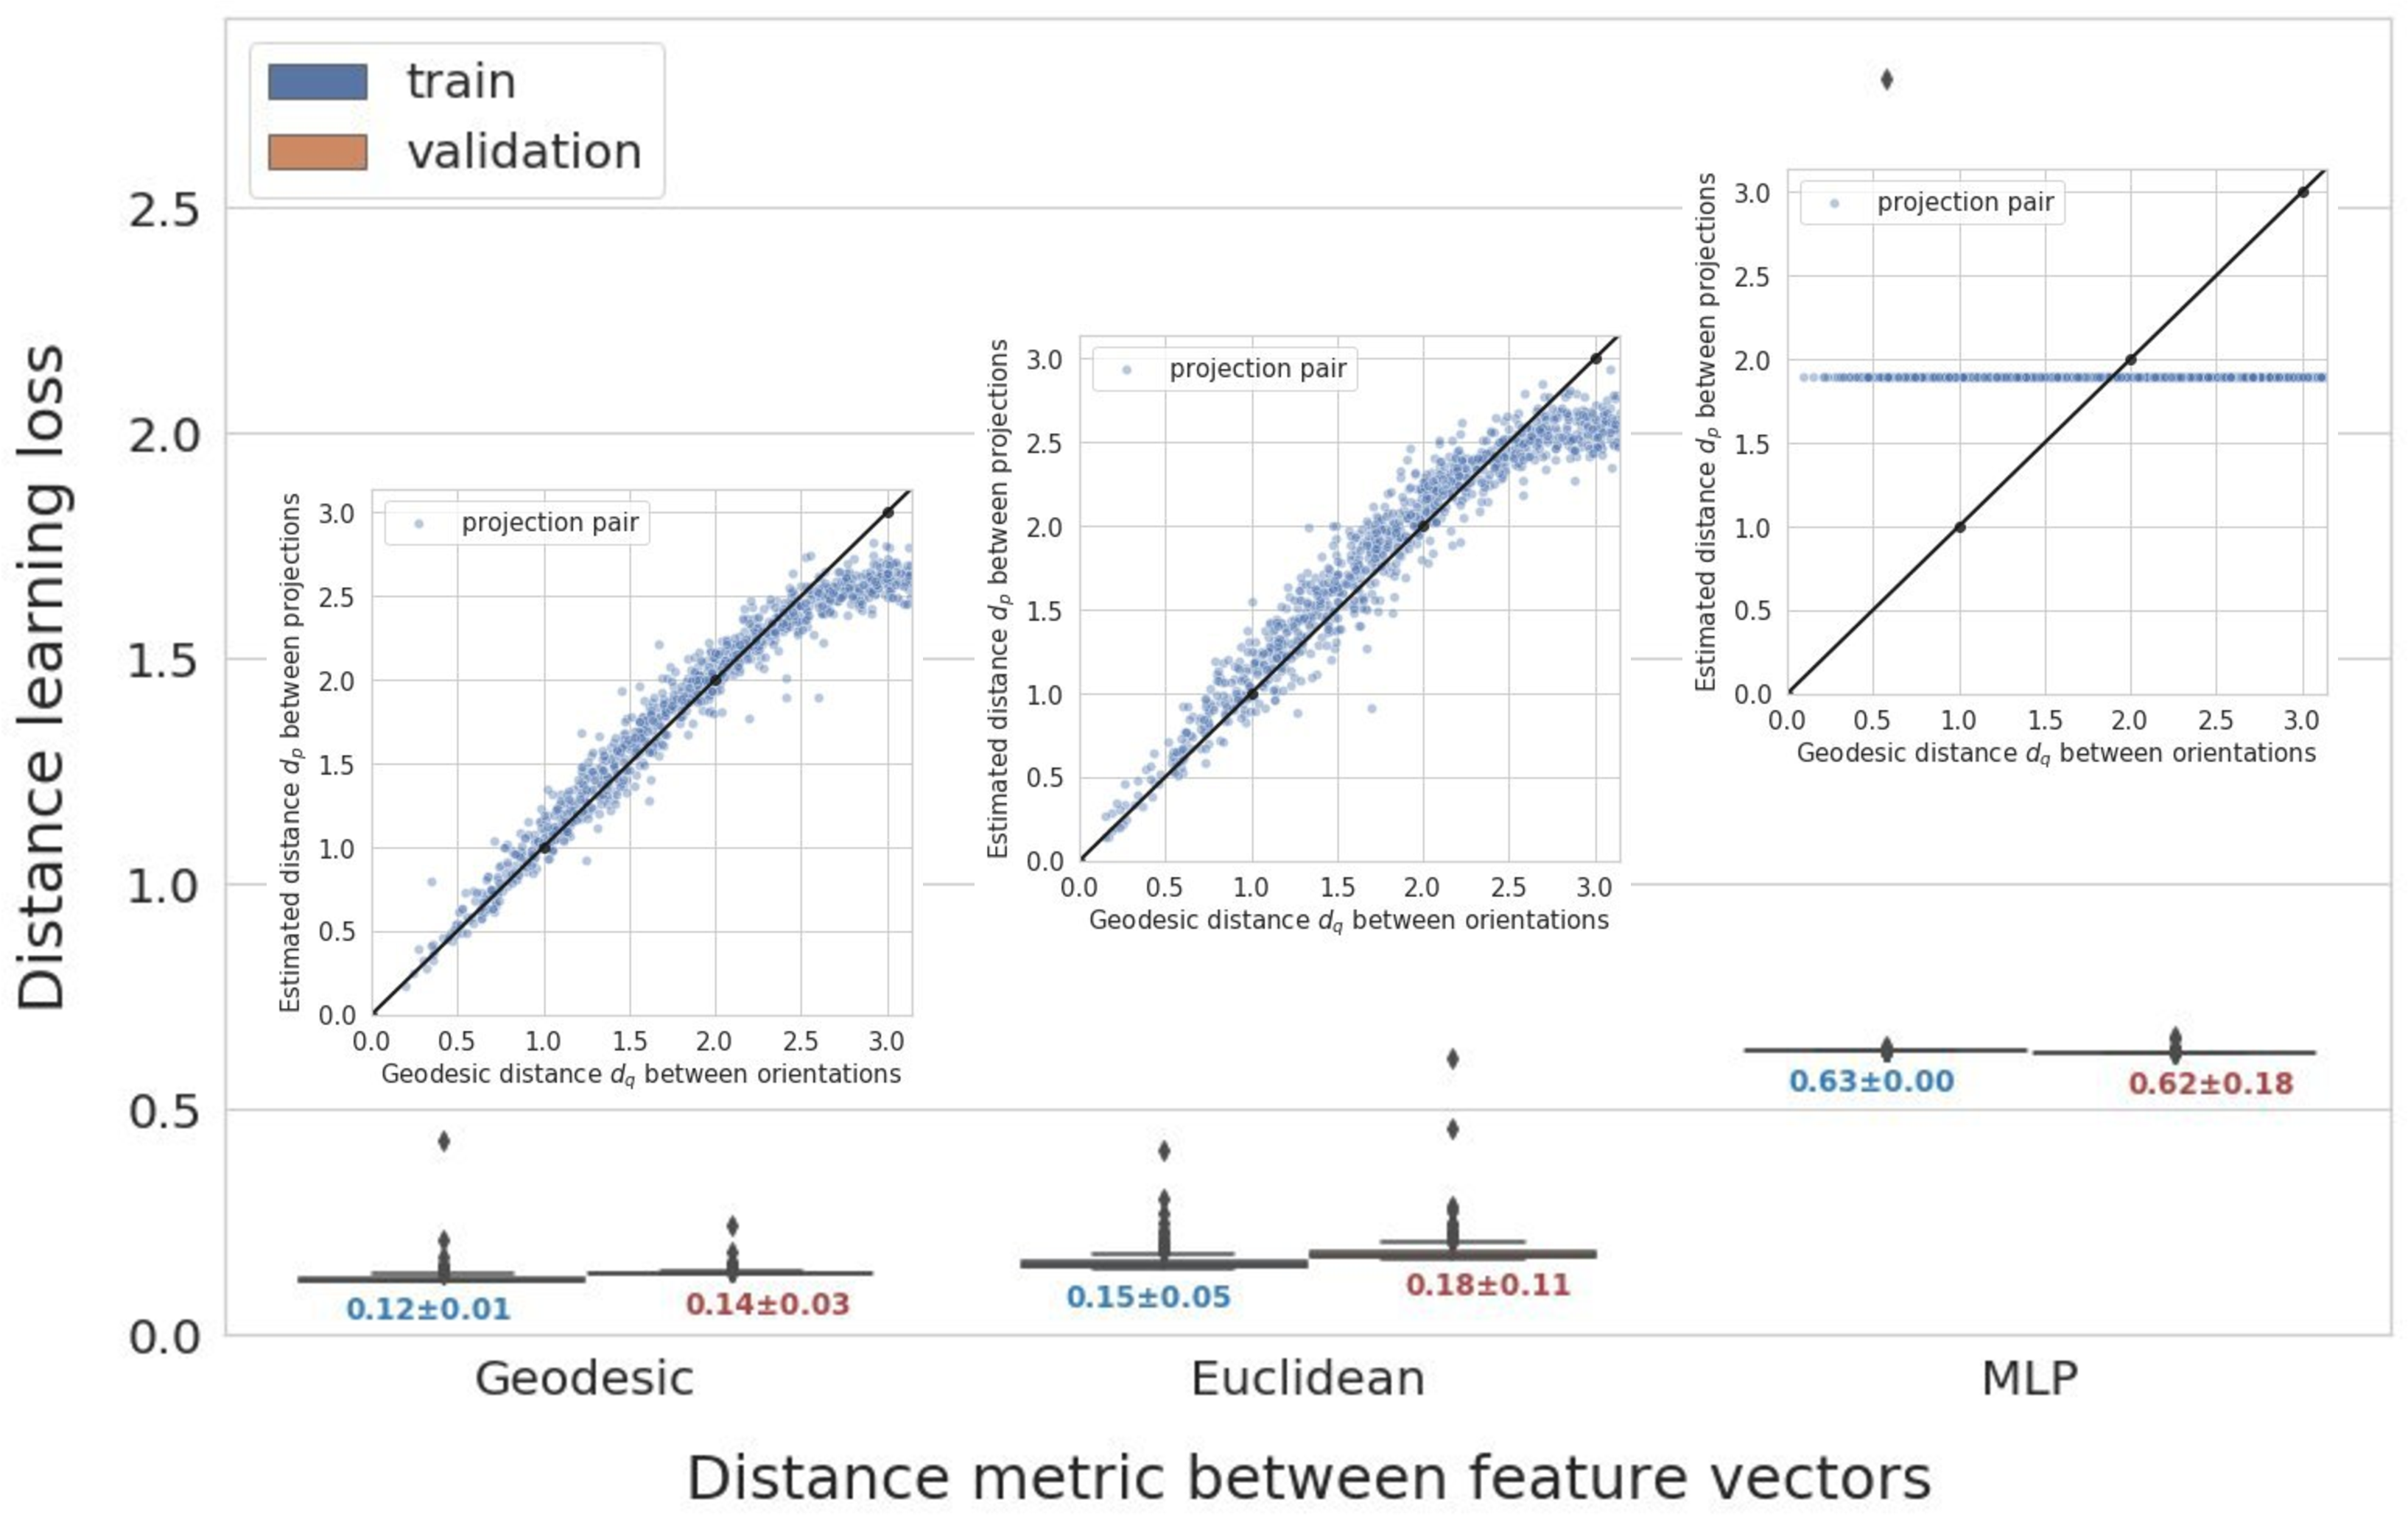
\includegraphics[height=4cm]{figures/geo_eucl_mlp_distance_metric.pdf}
        \caption{%
            Performance of distance learning w.r.t.\ the choice of feature distance function $d_f$.
            The box plots show the distance learning loss $L_\text{DE}$ \eqnref{distance-learning} on the training (blue) and validation (red) sets.
            The inserted plots show the relationship between $d_q(q_i, q_j)$ and $d_p(\p_i, \p_j) = d_f(\mathcal{G}_w(\p_i), \mathcal{G}_w(\p_j))$.
            \todo{Consistency: train -> training set, validation -> validation set, and Geodesic -> Cosine. Add $L_\text{DE}$ to the y-axis label. Larger text.}
            \todo{Remove the MLP results. It didn't work at all. Make the difference between Euclidean and Cosine easier to see.}
        }\label{fig:geo-eucl-mlp}
    \end{minipage}
\end{figure}

\section{Non-determinism of the Orientation Recovery}\label{apx:non-determinism}
\mdeff{Could we also have $E_\text{OR}$? It's easier to understand and compare.}
\banjac{I fully agree, however, I already mentioned that I wasn't able to align the orientations even though the $L_\text{OR}$ was very good. Looking at the estimation and GT in rotation space, it is visible we have some kind of transformation between these two (transformation similar to one we found the flip is causing, but it is not the flip).}
\mdeff{Right, thanks for explaining again. We should probably discuss that issue somewhere. An Appendix? Do we have examples when it worked and when it didn't?}
\banjac{Coming soon.}


\section{Choice of feature distance}\label{apx:feature-distance}

%\mdeff{Story: $d_f = d_q$ better than Euclidean and MLP $d_f$. }

There are multiple options for a distance function $d_f$ between two features $\mathbf{f}_i = \mathcal{G}_w(\p_i) \in \R^{n_f}$. We compared the performance of three different distances:

\begin{itemize}
    \item the Euclidean distance, i.e., $d_f(\mathbf{f}_i, \mathbf{f}_j) = \| \mathbf{f}_i - \mathbf{f}_j \|_2$
    \item the cosine distance, i.e.,
$ d_f(\mathbf{f}_i,\mathbf{f}_j) = 2 \arccos \left( \frac{\langle \mathbf{f}_i, \mathbf{f}_j \rangle}{\lVert \mathbf{f}_i \rVert \lVert \mathbf{f}_j \rVert} \right)$
\todo{No absolute value. So not as in \eqnref{distance:orientations}.}
    \item the parametrization of $d_f$ as a multi-layer perceptron (MLP) whose parameters are learned.
\end{itemize}

The MLP we tested was made of six layers with $1024, 512, 512, 256, 256, 1$ units, all of which use the SeLU activation function. The features $\mathbf{f}_i$ and $\mathbf{f}_j$ were stacked as an array of size $2n_f$ before being fed to the MLP\@. Note that, while a MLP can approximate any function, there is no guarantee that the learned function will satisfy the axioms of a proper distance function (i.e., the identity of indiscernibles, symmetry, and triangle inequality). \lau{Say that we were not able to train.}

\figref{geo-eucl-mlp} compares the use of the first two distances. The Euclidean distance yields better results, but the cosine distance is ultimately the best performer of all: $L_\text{DE}$ is the lowest, which makes $d_p$ a better estimator of $d_q$.
% the projection pairs deviate the least from the identity
This superiority of the cosine distance is likely due to its capacity to model the elliptic geometry of $\SO(3)$, a feat the Euclidean distance does not achieve, the Euclidean space being neither periodic nor curved.
%The $\SO(3)$ is non-linear and it can be explained with the fact that Euclidean distance of two quaternions can be small, despite the rotation being large~\cite{huynh_metrics_2009,DBLP:journals/corr/abs-1805-01026}.

\clearpage
\section{SiameseNN architecture}\label{apx:siamese-architecture}

% \begin{figure}[h!]
%     \centering
%     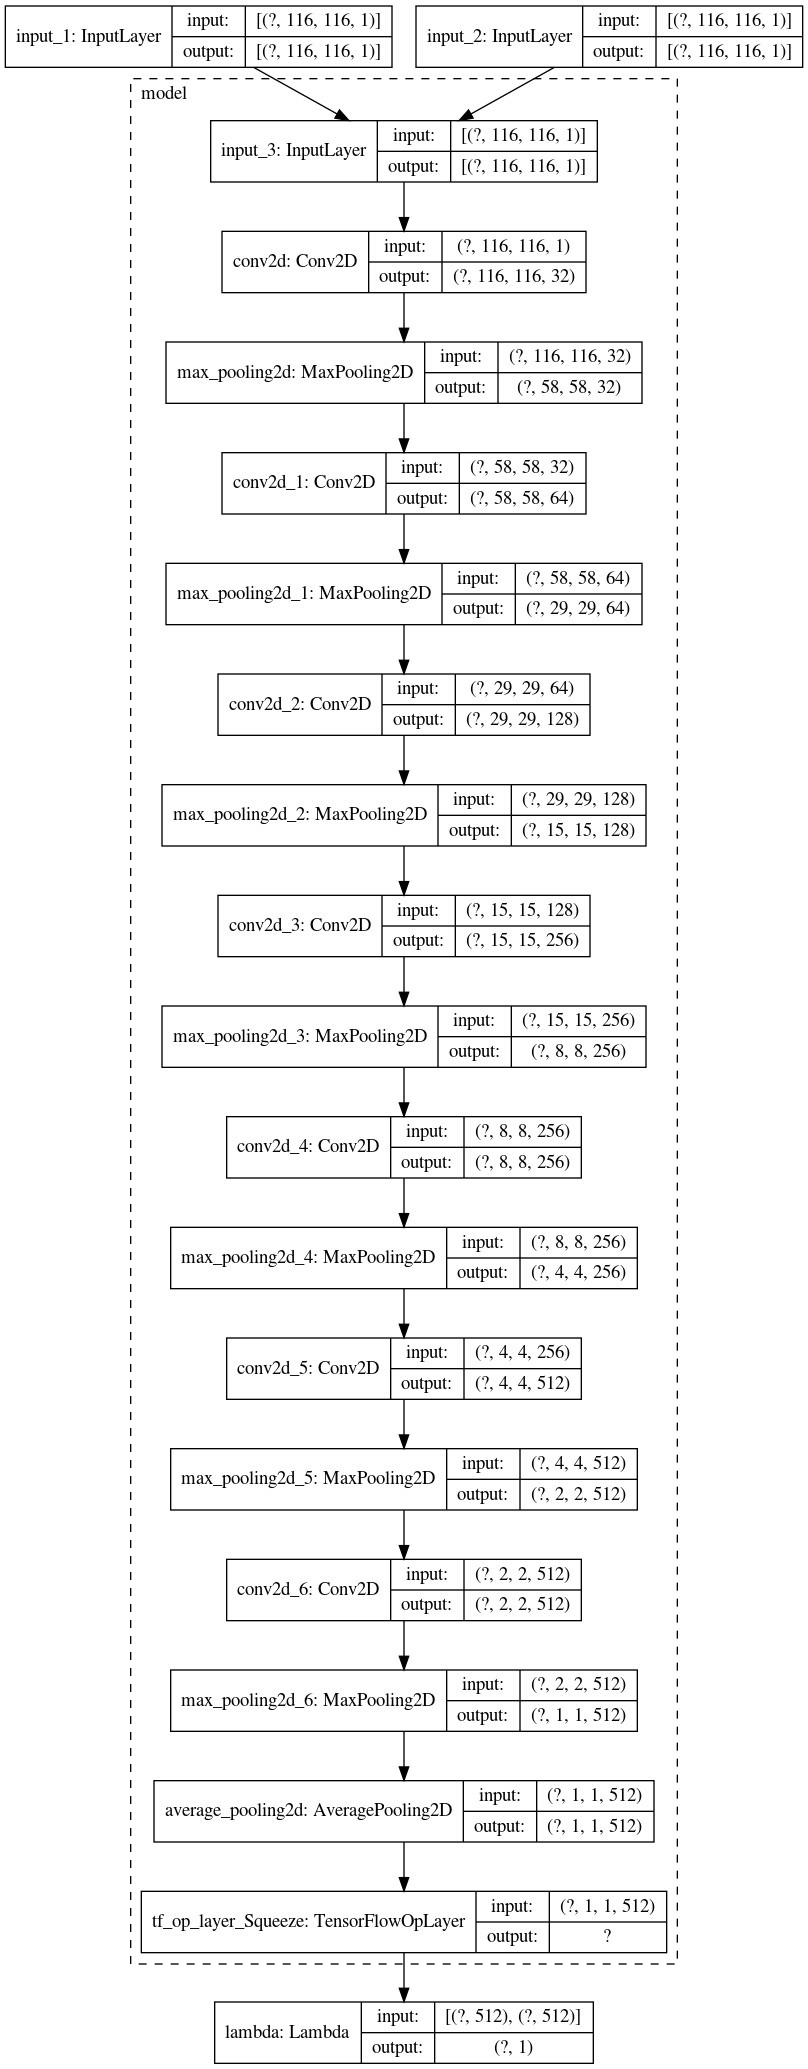
\includegraphics[height=19cm]{figures/model_plot.png}
%     \caption{%

%     }\label{fig:de-architecture}
% \end{figure}


\begin{figure}[ht!]
    \centering
    \begin{subfigure}[t]{0.47\linewidth}
        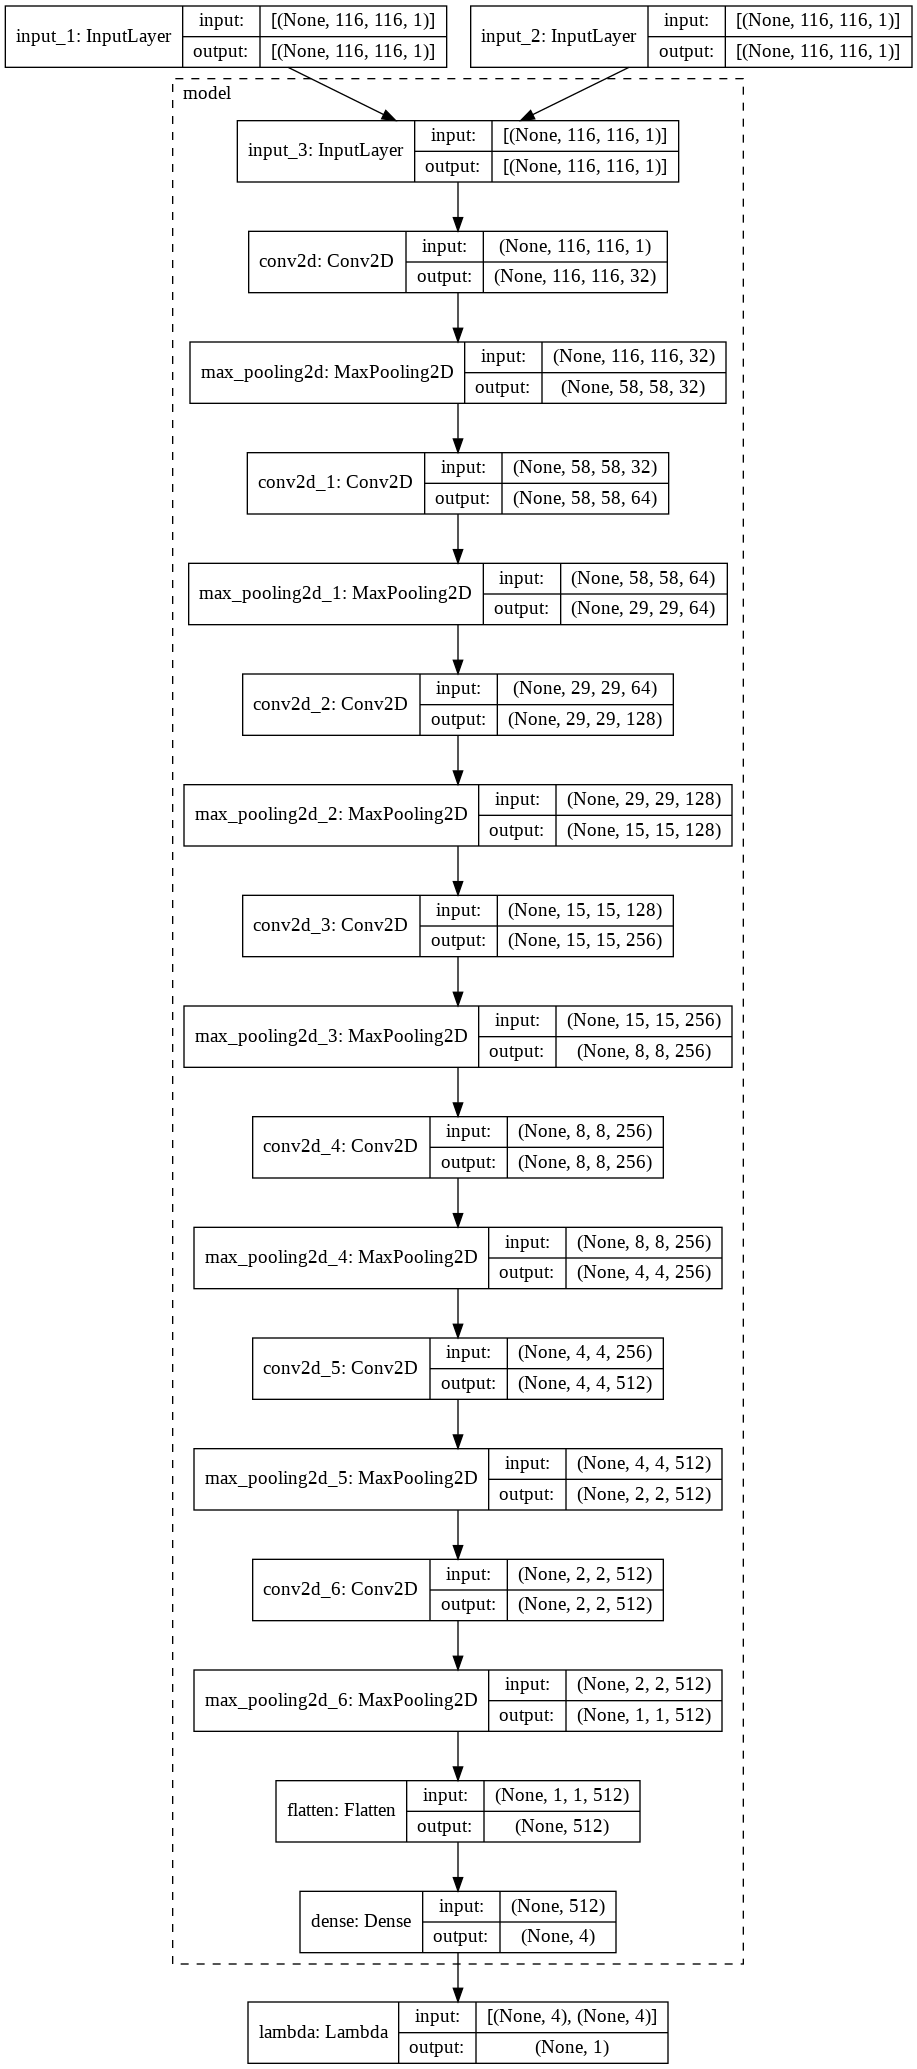
\includegraphics[width=\linewidth]{figures/model_plot_4d.png}
        \caption{%
           \banjac{Last layer converts feature vector to 4-dimensional vector.}
    }\label{fig:de-architecture:4d}
    \end{subfigure}
    \hfill
    \begin{subfigure}[t]{0.47\linewidth}
        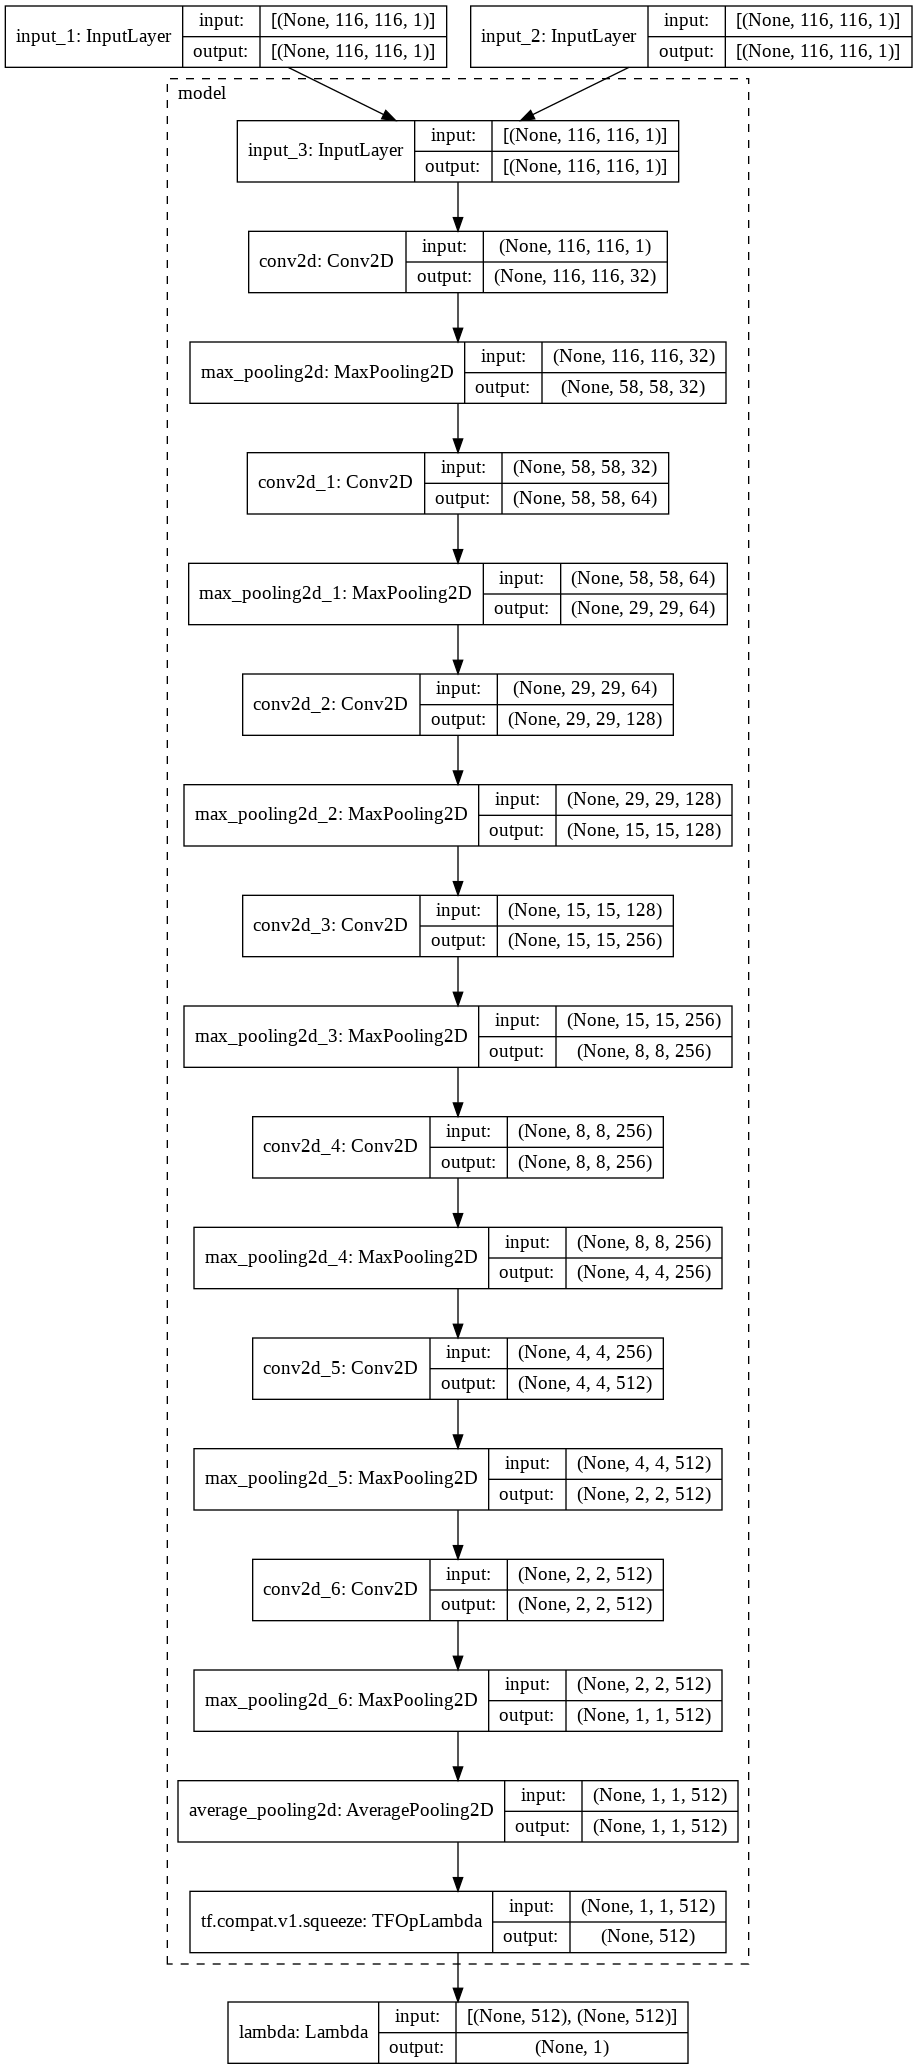
\includegraphics[width=\linewidth]{figures/model_plot_256d.png}
        \caption{%
           Last layer converts feature vector to a higher-dimensional vector of size 256. This architecture of network was used throughout all experiments.
        }\label{fig:de-architecture:256d}
    \end{subfigure}
    \caption{%
        Distance estimation network architecture.
        We have two input images of dimensions $116 \times 116$.
        Each one goes to its CNN (part where we share the weights, selected with a dashed line).
        The output is a scalar value representing the distance between these two images.
        \mdeff{Those are two similar to warrant two figures. We can just say that the last layer is different for $n_f=4$.}
    }\label{fig:de-architecture}
\end{figure}
